% chap2.tex
\part{유지보수 및 신기술 적용}
\label{part:module}

% ---------------------------------------------------------------------------- %
%                                  NEW SECTION                                 %
% ---------------------------------------------------------------------------- %

\chapter{pyGRsim 모듈}

\section{개발 원칙, 철학, 구조}

\subsection{철학}
음.. PEP8 따른다? 뭘 써야할지 고민 필요. @TODO

\subsection{전체 구조}
pyGRsim 밑에 core 있고 dragon 있고... core와 dragon은 동일한 하위폴더로 분류되어있고..

\subsection{환경 및 의존성}
이것도 위에서 몇 번 언급한 것 같은데 한 곳에서 통일할 필요가 있을듯.

% ---------------------------------------------------------------------------- %
%                                  NEW SECTION                                 %
% ---------------------------------------------------------------------------- %


\section{활용법}
python 레벨에서 이 모듈을 활용하려면 일단 GreenRetrofitModel을 직접 구축하는 예시부터 참고하면 됨.

% ---------------------------------------------------------------------------- %
%                                  NEW SECTION                                 %
% ---------------------------------------------------------------------------- %

\section{pyGRsim 구조별 상세}
pyGRsim이랑 dragon이랑 launcher랑 나누어서 서술할 것임.

\subsection{pyGRsim}
\subsubsection{construction}
구조임
\subsubsection{profile}
프로필임
\subsubsection{hvac}
시스템임
\subsubsection{shape}
모양?임
\subsubsection{model}
모델임

\subsection{dragon}
\subsubsection{construction}
구조임
\subsubsection{profile}
프로필임
\subsubsection{hvac}
시스템임
\subsubsection{shape}
모양?임
\subsubsection{model}
모델임
\subsection{imugi}
eppy를 대신하는 모듈. @TODO 어떤것을 위주로 사용되는지 서술 
\subsection{launcher}
EP 실행하는 모듈임. 모듈 구조는 아래와 같이 되어 있고, 향후 무슨무슨 실행을 고려할 수 있도록 구조화되었음. EP run 도는 부분까지 호출되는 순서는 유의 바람.
EP 돌아가는거 파싱하는 부분도 있음. 이런 가정 하에서 파싱하는거라서 혹시 이게 안되면 잘 안될지도 모름.

% ---------------------------------------------------------------------------- %
%                                  NEW SECTION                                 %
% ---------------------------------------------------------------------------- %

\section{데이터 변환의 구현}
\subsection{grexcel to grjson}
불러올 때 column들 filtering해서 들어오고 ID 붙이고...

\subsection{grjson to GreenRetrofitModel}
일단 reference하는 객체들이 있으니까 만들어놓고 dict에 저장하는 식으로 구현함. surface같은건 마지막에 ref관계 연결해줌. ref를 포함하는 얘들은 나중에 만드는 식으로 하고 fromjson함수에 그 dict들을 추가로 입력으로 받도록 해서 구현함

\subsection{GreenRetrofitModel to EnergyModel}
모든 GRM 객체는 to\_dragon을 가지고 있음 (zone 빼고). 그걸 가지고 하나씩 변환한다고 생각하면 됨. 일단 surface부터 만들어놓고 형상만들고 거기다가 설비를 갖다붙이는 순서로 만듬. 형상만들때 주의해야 하는게 아래 순서로 작업하는 걸 기억해야 함. 그리고 원본 훼손 안되게 해야 하니까 unknown인 얘들은 다시 복원해야 함.

\subsection{EnergyModel to idf}

\subsubsection{idf 기본 설정}
기본적으로 돌아가게 하기 위해서 아래 객체들을 먼저 만들어줘야 함.
\paragraph{Building} 필요함
\paragraph{SimulationOptions} 필요함

시뮬레이션 오류 없이 실행하기 위해 설정해야하는 class는 아래와 같음.
\paragraph{something} 을 설정해줘야함
\paragraph{something} 을 설정해줘야함
\paragraph{something} 을 설정해줘야함

\subsubsection{DB류 객체들 내보내기}
material, construction, profile 이런 것들은 미리 다 쌓아둔다.

\subsubsection{실재하는 객체들 하나씩 내보내기}
zone, surface, 설비같은 것들에 해당. 모든 EnergyModel 객체들은 다 to\_idf\_object 객체 가지고 있음. 기본적으로는 자기자신을 idfobject화 해서 계속 append하는 건데, 어떤 얘들은 좀 연동이 있어서 이걸 고려해야 함.

\subsubsection{후처리}
할 것들이 좀 있음

\subsubsection{ouptut 관리 등}
결과물 출력할 수 있게 작업해야 함

% ---------------------------------------------------------------------------- %
%                                  NEW SECTION                                 %
% ---------------------------------------------------------------------------- %

\section{EnergyPlus의 실행}
외부에서 입력이 들어오면, 그림 \ref{fig:eplaunchbycode}\와 같이 EnergyPlus가 호출됨
\begin{defaultfigure}
  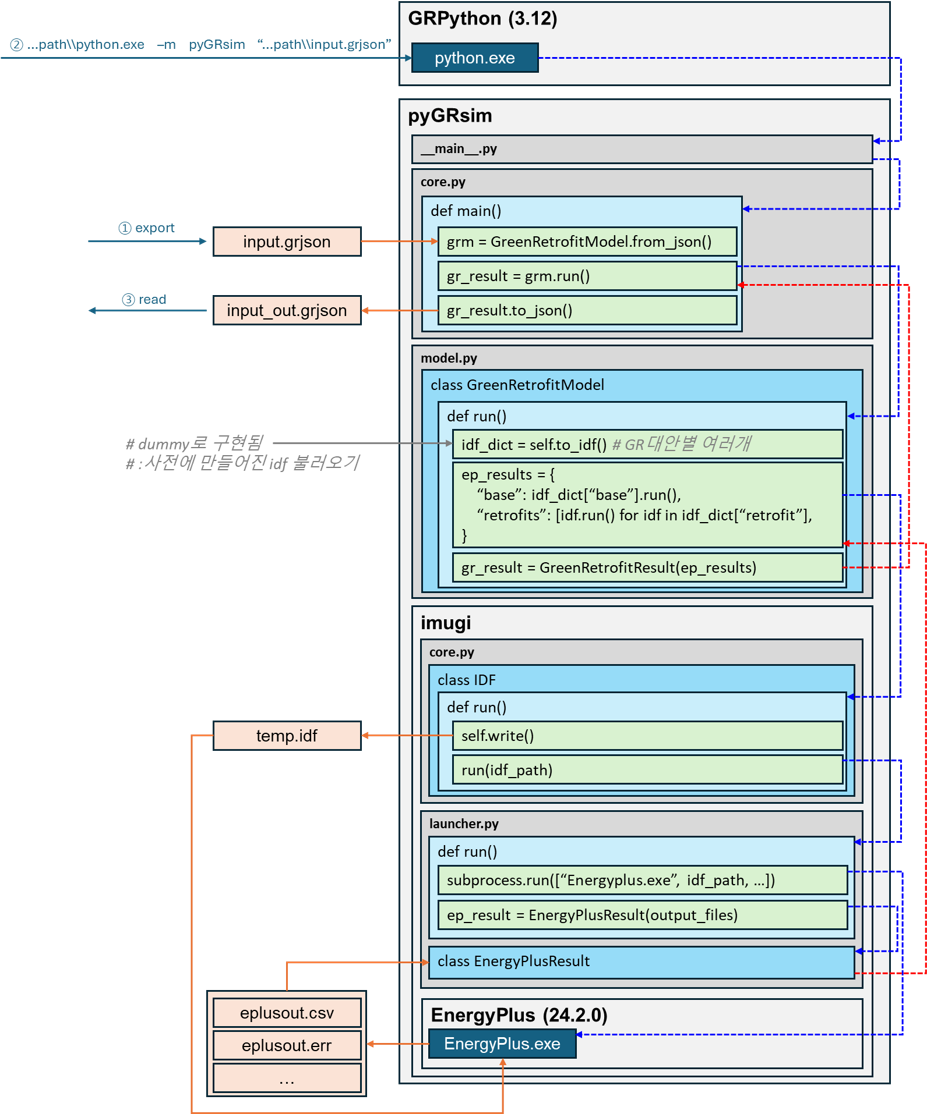
\includegraphics[height=0.99\textheight, width=\textwidth, keepaspectratio]{실행구조도.png}
  \caption{외부 호출 시 EnergyPlus launch되는 호출 흐름}
  \label{fig:eplaunchbycode}
\end{defaultfigure}

% ---------------------------------------------------------------------------- %
%                                  NEW SECTION                                 %
% ---------------------------------------------------------------------------- %

\section{예시코드}

import pyGRsim

% ---------------------------------------------------------------------------- %
%                                  NEW SECTION                                 %
% ---------------------------------------------------------------------------- %

\chapter{알고리즘의 수정과 코드의 유지보수}

\section{알고리즘의 수정 제안}

이런 값들을 바꿔보면서 수정하면 됨

% ---------------------------------------------------------------------------- %
%                                  NEW SECTION                                 %
% ---------------------------------------------------------------------------- %

\section{기본값 변경}

to\_idf\_object 

% ---------------------------------------------------------------------------- %
%                                  NEW SECTION                                 %
% ---------------------------------------------------------------------------- %

\section{일반적인 코드의 유지보수}

유지보수 방법

% ---------------------------------------------------------------------------- %
%                                  NEW SECTION                                 %
% ---------------------------------------------------------------------------- %

\chapter{신기술 적용}

\section{신기술의 시뮬레이터 적용하기 위해 필요한 개념적인 과정}

지금 체계에 맞아야 함. 예를 들어서,

% ---------------------------------------------------------------------------- %
%                                  NEW SECTION                                 %
% ---------------------------------------------------------------------------- %

\section{신기술을 본 시뮬레이터로 테스트해보는 방법}

idf에만 모듈 형식으로 결합할 수 있도록 작성. 일단 idf로 내보낸 다음에 신기술 override하고 결과해석 모듈 돌리는 방법이 있음.

% ---------------------------------------------------------------------------- %
%                                  NEW SECTION                                 %
% ---------------------------------------------------------------------------- %

\section{제도적으로 제출하기 위해 필요한 것}

이런 것들을 테스트하여 제출하기 바람. 테스트 건물은 우리가 쓴 것 쓰면 좋을 듯.